\documentclass[12pt]{article}
\usepackage[a4paper,left=2cm, right=2cm, top=2cm, bottom=2cm]{geometry}
\usepackage{graphicx}

\begin{document}
	\title{Assignment 2}
	\author{Meet Maratha}
	\maketitle
	\section{Problem Statement}
	The environment consists of 3 e-puck robots, out of which 2 are moving obstacles that move in a straight line. Other than them, there are 4 cylindrical obstacles in the environment and a start and goal position for the 3rd robot.
	\section{Method}
	The e-puck robot which needs to reach the goal uses the bug 0 algorithm for its movement. When it encounters an obstacle it encircles it in the left direction till it finds a line of sight to the goal. The other e-puck robots act as an obstacle for the above-mentioned robot. They move in a straight line with two points, which are chosen as the goal for them iteratively. These robots have a region of 0.5m around them where entering it is considered a collision. The size 0.5m is used after scaling a 2m radius to a smaller scale for visualization.
	\begin{figure}[h]
		\centering
		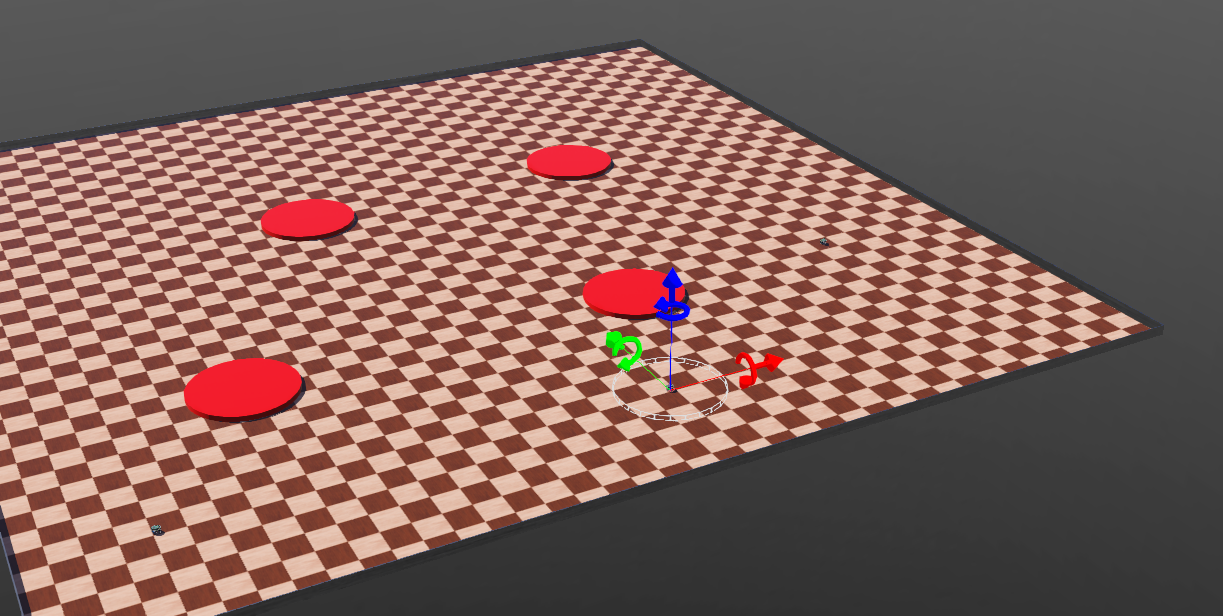
\includegraphics[scale=0.4]{images/Assignment 2.png}
		\caption{Webots Environment}
	\end{figure}
	
	\section{Conclusion}
	The robot reached the goal location successfully. The method can further be improved using a gradient field for path planning where a static gradient field is generated using 4 stationary obstacles and generating a gradient field for moving obstacles in each iteration and planning the next move based on it.
\end{document}